%!TEX encoding = UTF-8 Unicode

%!TEX root = ../compendium2.tex

\Lab{\LabWeekFIVE}

\begin{Goals}
%!TEX encoding = UTF-8 Unicode

%!TEX root = ../compendium2.tex

\item Kunna skapa en klass utifrån en textuell beskrivning. % av dess medlemmar.
%\item Kunna skapa en klass utifrån ofärdig kod och dokumentationskommentarer.
%\item Kunna införa privata attribut med lämpliga namn som representerar instansers förändringsbara tillstånd.
\item Kunna förklara skillnaden mellan klasser och instanser av klasser.
\item Kunna förklara skillnader och likheter mellan ett singelobjekt och objekt som är instanser av klasser.
\item Kunna förklara skillnaden mellan förändringsbara och oföränderliga objekt.
%\item Förstå innebörden av instansreferensen \code{this}.
\item Kunna skapa och använda klasser vars instanser innehåller referenser till andra instanser (aggregering).

\end{Goals}

\begin{Preparations}
\item \DoExercise{\ExeWeekFIVE}{05}

\item Läs igenom hela laborationen och studera dokumentationen för:
\begin{itemize}[nolistsep,noitemsep]
\item klassen \jcode{SimpleWindow} här: \url{http://cs.lth.se/pgk/api/}

\item \code{scala.Double} och \code{scala.math}, speciellt metoder för avrunding, trigonometri och polära koordinater, här:
\url{http://www.scala-lang.org/api/current/} 
\end{itemize}

\end{Preparations}

\subsection{Bakgrund}

Under den här laborationen ska du skapa en samling av klasser som tillsammans kan användas för att rita i ett fönster. Du ska bland annat skapa en klass \code{Turtle} som använder den färdigskrivna java-klassen \code{SimpleWindow} för att möjliggöra sköldpaddsgrafik liknande det vi gjorde i kojo-laborationen i avsnitt \ref{section:lab:kojo}. 

%SimpleWindow kan skapa ett enkelt ritfönster på skärmen, med metoder för att rita linjer, etc. SimpleWindow håller koll på en ''penna'' som representerar \textit{aktuell ritposition}. Det finns metoder för att flytta pennan och att rita en rak linje från pennans aktuella ritposition till en ny pennposition. 
%Delar av dokumentationen för SimpleWindow återspeglas i nedan specifikation. 
%Den fullständiga dokumentationen återfinns här: \url{http://cs.lth.se/pgk/api/}

%\vspace{1em}%hack to keep comment with method
%\begin{JavaSpec}{class SimpleWindow}
%  /** mouse click event type */
%	public final static int MOUSE_EVENT = 1;
%
%  /** key pressed event type */
%	public final static int KEY_EVENT = 2;
%
%  /** window closed event type */
%	public final static int CLOSE_EVENT = 3;
%
%  /** Creates a window and makes it visible. */
%	public SimpleWindow(int width, int height, String title);
%
%  /** Returns the width of the window. */
%	public int getWidth();
%
%	/** Returns the height of the window. */
%	public int getHeight();
%
%	/** Clears the window. */
%	public void clear();
%
%	/** Closes the window.*/
%	public void close();
%
%	/** Opens the window. */
%	public void open();
%
%	/** Moves the pen to a new position. */
%	public void moveTo(int x, int y) ;
%
%	/** Moves the pen to a new position while drawing a line. */
%	public void lineTo(int x, int y);
%
%	/** Writes a string at the current position.* /
%	public void writeText(String txt);
%
%	/** Draws a bitmap image at the current position.*/
%	public void drawImage(Image image);
%
%	/** Returns the pen's x coordinate. */
%	public int getX();
%
%	/** Returns the pen's y coordinate. */
%	public int getY();
%
%	/** Sets the line width.  */
%	public void setLineWidth(int width);
%
%	/** Sets the line color. */
%	public void setLineColor(Color col);
%
%	/**Returns the current line width. */
%	public int getLineWidth();
%
%	/** Returns the current line color. */
%	public Color getLineColor();
%
%	/**  Waits for a mouse click. */
%	public void waitForMouseClick();
%
%	/** Returns the mouse x coordinate at the last mouse click. */
%	public int getMouseX();
%
%	/** Returns the mouse y coordinate at the last mouse click. */
%	public int getMouseY();
%
%	/**Adds a sprite to the window. */
%	public void addSprite(Sprite sprite);
%
%	/** Wait for a specified time. */
%	public static void delay(int ms);
%\end{JavaSpec}
%
%
%\clearpage

\subsection{Obligatoriska uppgifter}


\Task Skapa dessa kataloger %(kallas även bibliotek eller mappar på svenska och \emph{''folder''} eller \emph{directory} på engelska) 
och tomma filer för din kod med hjälp av nedan linuxkommandon (eller motsvarande på annat lämpligt sätt):
\begin{REPLnonum}
mkdir turtle
cd turtle
mkdir -p src/main/scala/graphics
touch Point.scala Main.scala 
mv *.scala src/main/scala/graphics/.
ls src/main/scala/graphics/
\end{REPLnonum}
Om man skriver mycket kod blir det lättare att hitta olika delar om man har dem i olika filer med lämpliga  filnamn. Det är vanligt att man lägger kodfilerna i katalogen \code{src/main/scala} och där skapar en egen underkatalog för varje paket med samma namn som paketet.\footnote{Flera verktyg kräver exakt denna katalogstruktur för att hitta koden utan specialinställningar.} 


\Task Du ska skapa case-klassen \code{Point} som ska beskriva en koordinat i ett kartesiskt koordinatsystem\footnote{\url{https://sv.wikipedia.org/wiki/Kartesiskt_koordinatsystem}}. Skapa kod med hjälp av en editor, t.ex. \code{atom}, i filen  \code{src/main/scala/graphics/Point.scala} enligt följande riktlinjer:
\begin{enumerate}%[noitemsep]
\item Klassen \code{Point} ska vara en oföränderlig case-klass. 

\item Klassen \code{Point} ska ligga i paketet \code{graphics}.

\item Klassen \code{Point} ska ha följande två publika, oföränderliga klassparametrar:
\begin{itemize}[nolistsep, noitemsep]
\item \code{x: Double} för x-koordinaten.
\item \code{y: Double} för y-koordinaten.
\end{itemize}

\item Klassen \code{Point} ska ha följande publika medlemmar (två oföränderliga attribut och två metoder):
\begin{itemize}[nolistsep, noitemsep]
\item \code{val r: Double} ska ge motsvarande polära kordinatens%
\footnote{\url{https://sv.wikipedia.org/wiki/Pol\%C3\%A4ra\_koordinater}}
 avstånd till origo.
\item \code{val theta: Double} ska ge polära kordinatens vinkel i radianer.
\item \code{def negY: Point} ska ge en ny punkt med y-koordinaten negerad. 
\item \code{def +(p: Point): Point} ska ge en ny punkt vars koordinat är summan av x- respektive y-kordinaterna för denna instans och punkten \code{p}.
\end{itemize}

\item Klassen \code{Point} ska ha ett kompanjonsobjekt med en metod som konstruerar en punkt från polära koortdinater. Metoden ska ha detta huvud: \\\code{def polar(r: Double, theta: Double): Point}

\end{enumerate}

\noindent Tips vid implementation och senare användning:
\begin{itemize}
\item Du har nytta av metoderna \code{math.hypot(x, y)} och \code{math.atan2(y, x)} vid omvandling till polära koordinater.

\item Du har nytta av metoderna \code{math.cos(x)} och \code{math.sin(y)} vid omvandling från polära koordinater.

\item Attributet \code{negY} kommer att underlätta för dig när du i metoden \code{draw} i klassen \code{Turtle} ska omvandla en punkt till fönsterkoordinater där y-axeln är omvänd jämfört med kartesiska koordinater.

\item Notera att klassens attribut är av typen \code{Double} och inte \code{Int}, trots att vi senare ska använda punkten för att beskriva en diskret pixelposition. Anledningen till detta är att det kan uppstå avrundningsfel vid numeriska beräkningar. Detta blir särskilt märkbart vid upprepad räkning med små värden, t.ex. när man ritar en approximerad cirkel med många linjesegment.
\end{itemize}

\noindent Du ska kunna använda din punkt enligt följande exempel. Starta REPL och klistra in din case-klass med sitt kompanjonsobjekt efter kommandot \code{:paste} (eller kortare \code{:pa}). Du ska inte ta med paketdeklarationen då \code{package} inte fungerar i REPL.
\begin{REPLnonum}
scala> Point(1,1).theta.toDegrees
res0: Double = 45.0

scala> Point(3,4).r
res1: Double = 5.0

scala> Point(1,1).negY + Point(2,5)
res2: Point = Point(3.0,4.0)

scala> Point.polar(2, 60.0.toRadians).theta.toDegrees
res3: Double = 60.000001669652114
\end{REPLnonum}


\Task Lägg \code{cslib.jar} i katalogen \code{lib}, t.ex. med dessa linuxkommandon:
\begin{REPLnonum}
$ mkdir lib
$ wget -O lib/cslib.jar http://cs.lth.se/pgk/cslib
\end{REPLnonum}

\Task Skapa en \code{main}-metod i singelobjektet \code{Main} i paketet \code{graphics} i filen \code{src/main/scala/graphics/Main.scala} som gör något enkelt med både \code{Point} och \code{SimpleWindow}, t.ex. drar en linje mellan två punkter enlig nedan. 
\scalainputlisting[numbers=left,basicstyle=\ttfamily\fontsize{11}{13}\selectfont]%
{../workspace/w05_turtle/src/main/scala/graphics/Main.scala}

\noindent När många kodfiler beror av varandra behöver kompilatorn ha tillgång till alla kodfiler samtidigt.  Detta kan åstadkommas genom att ge \code{*.scala} som argument till \code{scalac} enligt nedan. Dessutom blir det en hel del \code{.class}-filer som utdata från kompilatorn, så man brukar lägga dem i en katalog med namnet \code{bin} (eller ibland \code{target}) för att separera dem från övriga filer. Använd följande linuxkommando\footnote{I Windows, byt ut kolon mot semikolon.} för att skapa \code{bin}-katalog, samkompilera alla filer och köra \code{main}-metoden:
\begin{REPLnonum}
$ mkdir bin
$ scalac -cp lib/cslib.jar -d bin src/main/scala/graphics/*.scala
$ scala -cp "lib/cslib.jar:bin" graphics.Main
\end{REPLnonum}


\Task Skapa klassen Turtle som representerar en virtuell sköldpadda med en penna under magen som kan rita i \code{SimpleWindow} enligt nedan riktlinjer:

\begin{enumerate}
\item Klassen \code{Turtle} ska vara en klass med ett förändringsbart tillstånd bestående av tre privata attribut som håller reda på detta:

\begin{itemize}
\item en position av typen \code{Point} där ett positivt y-värde räknas \emph{nedåt} i fönstret.
\item en riktning av typen \code{Double} som anges som en vinkel i grader  (och inte radianer), där ett positivt värde anger vinkeln motsols från x-axeln. 
\item ett läge på pennan av typen \code{Boolean} där \code{true} anger att pennan är nere.
\end{itemize}

\item Utgå från det ofärdiga kodskelettet nedan där dokumentationskommentarerna ger ytterligare detaljer att ta hänsyn till. Om du skriver klassen från början behöver du inte skriva av dokumentationskommentarerna. Kodskelettet finns annars i kursens \code{workspace} på GitHub%
\footnote{\url{https://github.com/lunduniversity/introprog/blob/master/workspace/}} och här: \url{http://cs.lth.se/pgk/ws}

\item Flera metoder har \code{Turtle} som returtyp. I dessa fall ska en referens till den egna instansen returneras för att möjliggöra upprepad punktnotation, t.ex.:\\
\code{t.jumpTo(Point(100, 200)).turnNorth.penDown}

\scalainputlisting[numbers=left,basicstyle=\ttfamily\fontsize{10}{12}\selectfont]%
{../workspace/w05_turtle/src/main/scala/graphics/Turtle.scala}
\end{enumerate}

\noindent Tips:

\begin{itemize}
\item Allteftersom du implementerar de saknade delarna, utöka din \code{main}-metod i \code{Main.scala} med fler tester och kolla så att dina implementationer funkar som det är tänkt. Testa på nytt efter varje litet tillägg så att du hela tiden har något som fungerar. Det är mycket lättare att felsöka efter en liten ändring än efter många och stora ändringar.

\item Du får namnge de privata variablerna som representerar det förändringsbara tillståndet så som du själv anser lämpligt. Tänk på att det i Scala kan bli namnkrock mellan metoder och privata attribut. I dessa fall brukar man namnge det privata attributet med ett understreck före för att skilja dem åt, t.ex.: \\
\code{private var _direction: Double  = ???}

\item I metoden \code{forward} har du nytta av metoden \code{Point.polar}, metoden \code{.toRadians} som kan konvertera en \code{Double} i grader till radianer, samt metoden \code{negY}. Tänk på att vinkelberäkningar på radianer förutsätter kartesiskt koordinatsystem, så negeringen av Y-axeln ska ske efter sådana beräkningar, men innan uppdatering av positionen sker. 
\end{itemize}


\Task Implementera case-klassen \code{Rect} enligt specifikationen nedan. Kodskelettet finns i workspace. Testa dina implementationer allteftersom du skriver dem, genom att stegvis utöka din \code{main}-metod.

\scalainputlisting[numbers=left,basicstyle=\ttfamily\fontsize{10.5}{12}\selectfont]%
{../workspace/w05_turtle/src/main/scala/graphics/Rect.scala}

\noindent Flera metoder ovan har \code{Rect} som returtyp. I dessa fall ska en referens till den egna instansen returneras för att möjliggöra upprepad punktnotation, t.ex.:\\
\code{r.rotatedLeft(15).translated(0, 2).scaled(1.5)}

\TODO{Gör så att draw och drawCentered också returnerar Rect???}

\clearpage

\Task\Checkpoint När \code{Turtle} och \code{Rect} är färdigimplementerade så ska du testa klasserna gemensamt genom att köra \code{main}-metoden i singelobjektet \code{Demo} nedan. Koden finns i kursens workspace. 

Den första bilden ska visa två lika stora rektanglar i samma höjd. Efter musklick kommer en animering av tre färgglada rektanglar. När det finns en handledare ledig, redovisa vad du åstadkommit. Vid väntetid, fortsätt med efterföljande uppgifter.

\scalainputlisting[numbers=left,basicstyle=\ttfamily\fontsize{11}{14}\selectfont]%
{../workspace/w05_turtle/src/main/scala/graphics/Demo.scala}


\clearpage

\subsection{Frivilliga extrauppgifter}

Nedan uppgifter kan göras i valfri ordning.

\Task Använd din Turtle för att rita en cirkel. För att göra detta kan du t.ex. låta din Turtle gå ett kort steg och svänga någon grad tills den har gjort ett fullt varv.

\Task Skapa två stycken Turtles i samma fönsterobjekt som rör sig alternerande. Fungerar allt som tänkt?


\Task Studera dokumentationen för de \code{SimpleWindow}-metoder som erbjuder hantering av händelser \Eng{event} och använd dessa för lösa deluppgifterna nedan.

\Subtask Gör så att en Turtle kan styras med hjälp av tangentbordstryckningar A--S--D--W för vänster--ner--höger--upp och att den ritar ett spår allteftersom den förflyttas.

\Subtask Gör så att en andra Turtle kan styras med hjälp av tangentbordstryckningar J--K--L--I för vänster--ner--höger--upp och att den också ritar ett spår allteftersom den förflyttas.

\Subtask Gör så att, när de två sköldpaddorna ovan befinner sig tillräckligt nära varandra, det ritas ut en rektangel med hörn där de två sköldpaddorna finns. (Denna uppgift är lite svårare och kan behöva delas upp i delar.)


\Task Studera dokumentationen för de \code{SimpleWindow}-metoder som erbjuder hantering av flyttbara bilder \Eng{sprites}. Gör så att en fin Sprite ritas vid positionen för de styrbara sköldpaddorna i föregående uppgift.


\Task Skapa en case-klass \code{RectSeq} enligt specifikation på sidan \pageref{code:classes:graphics:rectanglesequence}. I denna klass skall metoden \code{draw} rita ut ett antal rektanglar där varje rektangel har förflyttat sig, roterats och skalats jämfört med föregående rektangel i sekvensen. 

\begin{figure}[H]
\centering
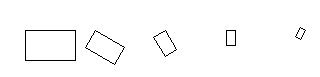
\includegraphics[width=0.75\textwidth]{../img/turtle/RectSeq.png}
%\caption Rotation av rektangel med koden nedan.
%\label{fig:classes:graphics:rollingrectangle}
\end{figure}
\noindent Bilden ovan kan skapas med hjälp av denna kod:
\begin{Code}
  def rectSeqExample(t: Turtle): Unit  = {
    val rect = Rect(pos = Point(200, 200), width = 50, height = 30)
    RectSeq(rect, n = 5, dist = 70, rot = -30, scale = 0.67).draw(t)
  }
\end{Code}

\noindent Nedan kod ritar bilden i fig. \ref{fig:classes:graphics:rectanglesequence} på sidan \pageref{fig:classes:graphics:rectanglesequence}. Använd gärna \code{setLineColor} i \code{SimpleWindow} för att göra en färggladare stjärna. Slumpvisa transformationer är också kul. 

\begin{Code}
val w = new SimpleWindow(500, 500, "Shapes")
val t = new Turtle(w, new Point(200, 200), 0, false)
val rect = Rect(pos = Point(225, 235), width = 50, height = 30)
val roll = RectSeq(rect, n = 100, dist = 2, scale = 0.98)
for (i <- 0 to 360 by 20) roll.rotatedLeft(i).draw(t)
\end{Code}


\begin{figure}
\centering
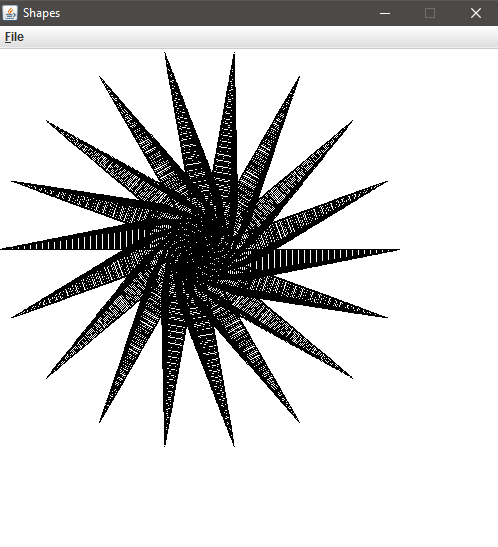
\includegraphics[width=0.5\textwidth]{../img/w06-lab/RectangleSequence.png}
\caption {En stjärna skapad med hjälp av \code{RectSeq}.}
\label{fig:classes:graphics:rectanglesequence}
\end{figure}

\noindent Nedan finns ett kodskellett som du kan utgå ifrån. Dokummentationskommentarerna innehåller fler detaljer om hur det är tänkt att klassen ska fungera. %De metoder som returnerar \code{RectSeq} ska returnera en referens till den egna instansen så att upprepad punktnotation möjliggörs.

\begin{figure}[H]
\scalainputlisting[numbers=left,basicstyle=\ttfamily\fontsize{9.9}{12}\selectfont]%
{../workspace/w05_turtle/src/main/scala/graphics/RectSeq.scala}
\label{code:classes:graphics:rectanglesequence}
\end{figure}



%\Task En riktig utmaning, för den som har lust: Implementera spelet ''Masken'' som beskrivs här: \url{https://sv.wikipedia.org/wiki/Snake}.
